
%
%  $Description: Author guidelines and sample document in LaTeX 2.09$
%
%  $Author: Gediminas Mazrimas $
%  $Date: 1995/09/15 15:20:59 $
%  $Revision: 1.4 $
%

\documentclass[times, 10pt,twocolumn]{article}
\usepackage{latex8}
\usepackage{times}

% Images includes
\usepackage{graphicx}
\usepackage{float}

%\documentstyle[times,art10,twocolumn,latex8]{article}

%-------------------------------------------------------------------------
% take the % away on next line to produce the final camera-ready version
\pagestyle{empty}

%-------------------------------------------------------------------------
\begin{document}

\title{Animating human model in OpenGL using data from Vicon system}

\author{Gediminas Mazrimas\\
Aalborg University Copenhagen\\ Computer Vision and Graphics\\g.mazrimas@gmail.com
\and
Algirdas Beinaravicius\\
Aalborg University Copenhagen\\ Computer Vision and Graphics\\algirdux@gmail.com
}

\maketitle
\thispagestyle{empty}

\begin{abstract}
   This paper explains how to animate 3D human model in OpenGL,
   avoiding most common problems, that occurs while dealing with
   various human body rigid parts transformations.
   The animation is associated with real person movements,
   while using data from Vicon motion capture system.
   Animating is made in lowest programming C++ OpenGL level.
   \\\\
   \textbf{Keywords:} Human animation, Vicon system, OpenGL, C++, Linear Blend Skinning
\end{abstract}



%-------------------------------------------------------------------------
\Section{Introduction}

Our animation focuses on the most common and partly simple human
body animation technique, that uses joints to animate human model. The joint structure,
given their position and orientation, can be thought as being human body skeleton.
The skin shape is associated to the joints, where as it's a 3D polygon mesh
and it's the only thing that is displayed for the end-user.
Due to very fast computation speeds, this technique is the most popular
in animation production. On the other hand, using simple shape blending technique
to deal with complex human body rigid parts transformations, there are
various skin deformation problems. Typical ones are collapsing elbow, candy-wrapper joint
when the arm turns 180 degrees, intersection between two adjacent bones (links) around a joint.
Also such a technique don't consider many very complicated and detail human body deformations,
for example dealing with muscles (stretch or bulge).

%-------------------------------------------------------------------------
\SubSection{Previous works}

What we've read and what was written there. References.
[Linear blend skinning, for deformation problems, data formats]

%-------------------------------------------------------------------------
\SubSection{Overview}

What is represented in further sections?

%-------------------------------------------------------------------------
\Section{Linear blend skinning}

Linear blend skinning technique is widely used for interactive applications.
It goes by many different names, such as Skeleton Subspace Deformation or SSD or smooth skinning" in Maya.

The linear blend skinning algorithm works by first placing a hierarchical
skeleton inside a static model mesh of a character in
some neutral pose (usually in the da Vinci posture or so called "dress pose").
Then, each vertex is assigned a set of influencing joints and a
blending weight for each influence. Computing the deformation in
some pose involves rigidly transforming each dress pose vertex by
all of its influencing joints. Then the blending weights are used to
combine these rigidly transformed positions.

The deformed vertex position, $ \overline{\textbf{v}} $ is
\begin{center}
$ \overline{\textbf{v}} = \displaystyle\sum_{i=1}^n\emph{w}_{i}M_{i}D_{i}^{-1}\textbf{v}_{d} $
\end{center}
where $w_{i}$ are the influence weights, $v_{d}$ is the dress-pose location of a
particular vertex \textbf{v}, $\emph{M}_{i}$ is the transformation matrix associated with
the $\emph{i}$th influence, and $D_{i}^{-1}$ is the inverse of the dress-pose matrix
associated with the $\emph{i}$th influence. Taken together, $D_{i}^{-1}\textbf{v}_{d}$ represents
the location of \textbf{v$_{d}$} in the local coordinate frame of the $\emph{i}$th influence.

\begin{figure}[H]
  \centering
  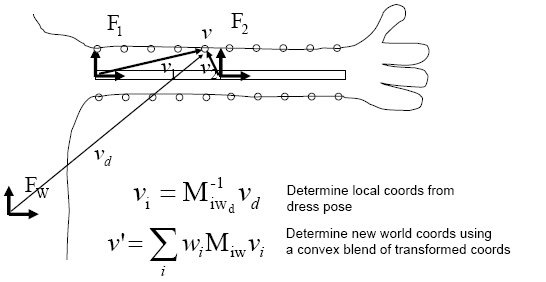
\includegraphics[width=93mm]{images/hand.jpg}
\end{figure}

Linear blend skinning though has two primary failings.
First, the method is incapable of expressing complex deformations.
Artifacts such as the "candy-wrapper", collapse effect on wrists and
collapsing around bending joints as shown appear. They
occur because vertices are transformed by linearly interpolated matrices.
If the interpolated matrices are dissimilar as in a rotation of
nearly 180 degrees, the interpolated transformation is degenerate,
so the geometry must collapse.
Second, authoring linear blend skins is difficult and frustrating for users.

Despite its failings, this skinning algorithm is very fast and
widely supported by commercial applications so it remains popular
especially in games and virtual environments.

%-------------------------------------------------------------------------
\Section{Vicon motion capture system}

What's Vicon motion capture system. How it works, what from it consists?

%-------------------------------------------------------------------------
\SubSection{Setting up system}

How we set up this system to be able to work with it.
How we prepare working space, how cameras are calibrated and similar.

%-------------------------------------------------------------------------
\SubSection{Capturing data}

How we capture our motion data (with costume). How we assign (label)
captured data to a Vicon model. How Vicon model looks like
(available joints, their connections, connections to costume sensors).

%-------------------------------------------------------------------------
\Section{Motion data}

What Motion data formats are we using? How do they look like?

%-------------------------------------------------------------------------
\SubSection{Description of Vicon C3D format}

This section is meant to give just a brief introduction to the C3D file format, describing it in an abstract way. A reference to a detailed manual, describing the format, is given in the reference part of this document.

The C3D (Coordinate 3D) file format is a binary data file format originally developed for the AMASS photogrammetry software system, capable of storing 3D data as well as analog data together with all associated parameters for a single measurement trial. Since only the 3D data is of importance, we will not consider analog data in this document. The main advantage of C3D format over other motion capture data formats is that it is able to encapsulate the motion data as well as parameters, describing the  motion data, in a single file. Apart from that, C3D is freely licensed and well documented.

Being a binary file, the C3D file consists of a number of 512-byte blocks. Logically C3D format can be divided into 3 basic sections, each having one or more 512-byte blocks:

    Header section is the first section of a file. The main purpose of this section is holding a pointer to the start of parameters section. Other parts of this section, is of no particular importance, as usually it consists data, copied from parameters section.

    The parameters section usually starts at block number 2, although this is not fixed and should not be assumed to be the case for every C3D file. This section contains information about the 3D data stored in the file. The section is extensible, meaning that user can define it's own parameters without  violating the format specification.

    Data section containing the 3D point coordinates is usually located after the parameters section. This section simply contains sequential frames data. In the case of 3D points (the data is X, Y and Z coordinates).

During the workflow of our project, the animation data, produced by the Vicon motion capturing system, was encoded in C3D file format. The data, provided by the C3D file, contains only the positions of skeleton joints at each frame, what is not sufficient to correctly animate the character. So the C3D animation data file was imported to Motion Builder, where the inverse kinematics technique was applied to provide us with BVH format file.  The BVH format file is another motion capturing data format, where the rotation data of each joint is being already calculated.


%-------------------------------------------------------------------------
\SubSection{Description of Biovision BVH format}

The BVH format is an updated version of BioVision�s BVA data format, with the addition of a
hierarchical data structure representing the bones of the skeleton.
The BVH file is an ASCII file and consists of two parts.

First section (HIERARCHY) is for storing hierarchy and initial pose of the skeleton,
basically joint-to-joint connections and offsets.
While as second section (MOTION) describes the channel motion data for each frame,
that is describes the movement of individual joints.

The HIERARCHY section starts with ROOT joint and contains OFFSET, CHANNELS and children JOINTS data.
Here OFFSET is followed by X, Y and Z coordinates, to determine current joint position.
CHANNELS information contains the existence of corresponding XYZ data streams (i.e. rotation and translation)
in the MOTION section which follows.
Finally it includes other JOINTS in hierarchical order with OFFSET and CHANNEL
and possible END SITE attribute, to determine body segment end.

In the MOTION section, each row contains data values for all CHANNELS which were specified in the HIERARCHY.
The listing order of CHANNELS values in each row in is assumed to match their listed order from the HIERARCHY section (top down).

There are only few drawbacks of this format, for example - the lack of a full definition of the basis pose
(it has only translational offsets of children segments from their parent, no rotational offset is defined)
and also it lacks explicit information for how to draw the segments,
but that has no bearing on the definition of the motion.

[Give more details later about exact structure of our model (like example)]

%-------------------------------------------------------------------------
\SubSection{Processing captured data}
Why do we need to convert C3D data to BVH?
What's good and bad about them? (C3d would be faster,
but it's binary, so not a human readable,
also BVH gives us rotations and have good structure,
that is much easier to implement in our C++ program).
How do we do it using Motion builder?


While C3D gives us our marker coordinates from motion capture system,
by labeling these markers at first in Vicon system and then importing them
in Motion builder, in BVH then we get rotations and translations not for those
markers, but for human body model joints.

[Here goes how we interpret BVH data]


%-------------------------------------------------------------------------
\Section{Human body mesh model}

What do we use for our animation?

%-------------------------------------------------------------------------
\SubSection{Mesh model preparations in Maya}

What Mesh model in Maya do we use?
How do we prepare it, that it would be suitable for out program?
How we cut mesh to different body parts, export to .obj format files.

%-------------------------------------------------------------------------
\SubSection{Mesh model file format used in animation}

Why do we use .obj file format? How does it look like?


%-------------------------------------------------------------------------
\Section{Animating human body}

Explain how we load human model, exported from Maya to .obj file.
How we create natural primary human pose, assign meshes to joints and so on.

%-------------------------------------------------------------------------
\SubSection{Loading human body model in OpenGL}

How we load human body to OpenGL. How we import mesh from obj files.
Joint creation. Joint connection with meshes.

%-------------------------------------------------------------------------
\SubSection{Linear blend skinning relations}

How we adapted linear blend skinning to our animations.
Explain how our method using meshes assigned with joint rotations
is similar to linear blend skinning. How we automated all the things.


%-------------------------------------------------------------------------
\Section{Conclusion}
Conclusion

%-------------------------------------------------------------------------
\nocite{ex1,ex2,ex3,ex4}
\bibliographystyle{latex8}
\bibliography{latex8}

\end{document}

